\documentclass{article}
% translate with >> pdflatex -shell-escape <file>

% This file is an extract of the PGFPLOTS manual, copyright by Christian Feuersaenger.
% 
% Feel free to use it as long as you cite the pgfplots manual properly.
%
% See
%   http://pgfplots.sourceforge.net/pgfplots.pdf
% for the complete manual.
%
% Any required input files (for <plot table> or <plot file> or the table package) can be downloaded
% at
% http://www.ctan.org/tex-archive/graphics/pgf/contrib/pgfplots/doc/latex/
% and
% http://www.ctan.org/tex-archive/graphics/pgf/contrib/pgfplots/doc/latex/plotdata/

\usepackage{pgfplots}
\pgfplotsset{compat=newest}

\pagestyle{empty}

\begin{document}

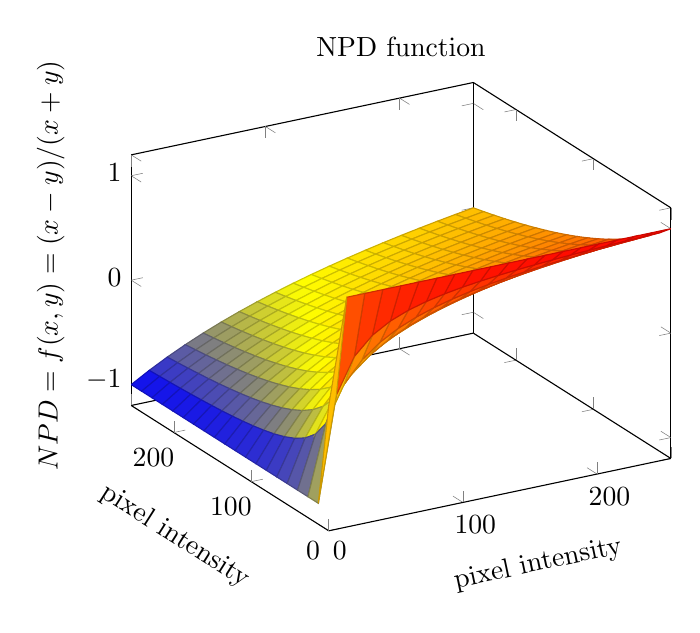
\begin{tikzpicture}
	\begin{axis}[
	title={NPD function},
	view/h=-30,
	view/az=-30,
	xlabel=pixel intensity,
	ylabel=pixel intensity,
	zlabel={$NPD=f(x,y)=(x-y)/(x+y)$},
	xlabel style={sloped like x axis},
	ylabel style={sloped}
	]
	\addplot3[surf,shader=faceted,
		samples=20,domain=0:255] 
		{(x-y)/(x+y)};
	\label{pgfplots:NPD}
	\end{axis}
\end{tikzpicture}
 \ref{pgfplots:label1} 

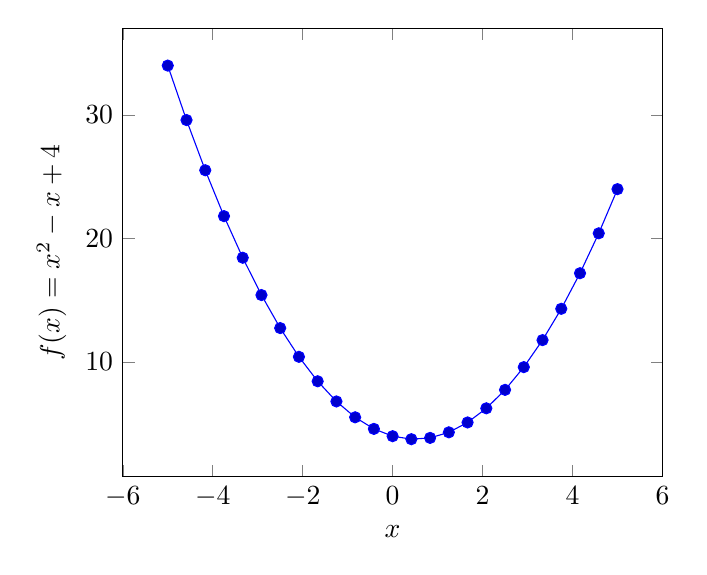
\begin{tikzpicture}
	\begin{axis}[
		xlabel=$x$,
		ylabel={$f(x) = x^2 - x +4$}
	]
	% use TeX as calculator:
	\addplot {x^2 - x +4};
	\end{axis}
\end{tikzpicture}


\end{document}
